\documentclass[a4paper,11pt]{article}
\usepackage[utf8x]{inputenc}
\usepackage[cm]{fullpage}
\usepackage{comment}
\usepackage{graphicx}
\usepackage{listings}
\lstset{language=Java, numbers=left, stepnumber=1, frame=single,}
\usepackage{hyperref}

%opening
\title{475 - Advanced Topics in Software Engineering \\ Acme Telecom}
\author{Ramie Al-Omari \texttt{ra808}, Dan Cooke \texttt{dc408}, Jonathan Evans \texttt{je08}, Javad Moghisi \texttt{jm308}}

\begin{document}
\maketitle

Our client requested a minor modification to a simple, but vital mobile phone customer billing system; the current charging criteria charges customers peak rate for the entire duration of their call if any part of the call falls within a peak period. New regulations stipulate calls must be charged at peak rate only for the time spent within a peak period. This report examines our approaches and techniques used to safely modify and enhance the existing legacy codebase.

We quickly learned there was no documentation present (formal, tests or code comments). This presented us with a major problem; an unknown existing system specification. The requirements specified that other than the stipulated modification, all other functionality should remain unchanged. Clearly the existing functionality would need to be accurately specified to ensure this condition is met. Thus our first goal was to develop a clear specification of the existing system, to allow us to safely refactor the codebase.

We began by implementing a Runner class with a main method to exercise various functionality within the system. We used debugging of this entry point to give us a better grasp of the existing system behaviour and flow. Inspecting the BillingSystem class, we quickly identified the part of the code that calculated the call charges. However, we did not make any changes to this and instead the initial workload was split between the group into writing acceptance tests using the FitNesse framework, writing Integration Tests with JUnit and setting up a developer workflow that included build and dependency management as well as a Continuous Integration (CI) server.

We assumed that the deadline for delivering the functionality to comply with the new regulations, coincides with the coursework submission deadline. Therefore, our first priority was to ensure that these requirements would be met in a safe and timely manner.


\section{Acceptance Testing}
To specify the functionality of the new system we wrote acceptance tests that captured both the new requirements and the remaining, unchanged behaviour of the old system. As there was no formal specification we had to be careful that these captured the full behaviour of the system. These tests are for testing that the system meets its specification rather than explicitly testing the output of the system (e.g. HTML markup isn't relevant).

We specified the following behaviour for calculating call costs of calls that:
\begin{itemize}
\item start and finish during the same peak/off-peak period
\item start during one peak/off-peak period and finish at the following peak/off-peak period
\end{itemize}
These cases would capture both the new requirements, i.e. calls with overlapping time periods, and the specification of part of the existing system, i.e. calls within the same time period.

We implemented the acceptance tests using Fit documents and executed them using the FitNesse acceptance testing framework. We decided to use Fit documents to specify the system as they can easily be edited and read by non-technical stakeholders at AcmeTelecom whilst FitNesse allows them to modify, view and run the tests using a user friendly Wiki interface. 

Our Fit documents followed the 'Given, When, Then' structure popular in behaviour-driven development. It allowed us to form behaviour 'narratives' that used domain language in a natural way that the client can understand. The tests were data driven and the 'Given' section permitted us to easily specify the information required by the test and meant that we did not rely on production data. FitNesse's ability to include other Fit documents as part of a test was particularly useful as it meant that customer and tariff data sets could be reused across all the tests.

An example of a Fit test that we created can be seen below. It is used to verify the correct billing rate is applied to calls made during off-peak calls but then overlap with the peak period. Although not strictly necessary given our set up and FitNesse fixtures, we decided to include the same tests for each of the three Tariffs because we felt that the client would find them easier to understand and follow.

\begin{center}
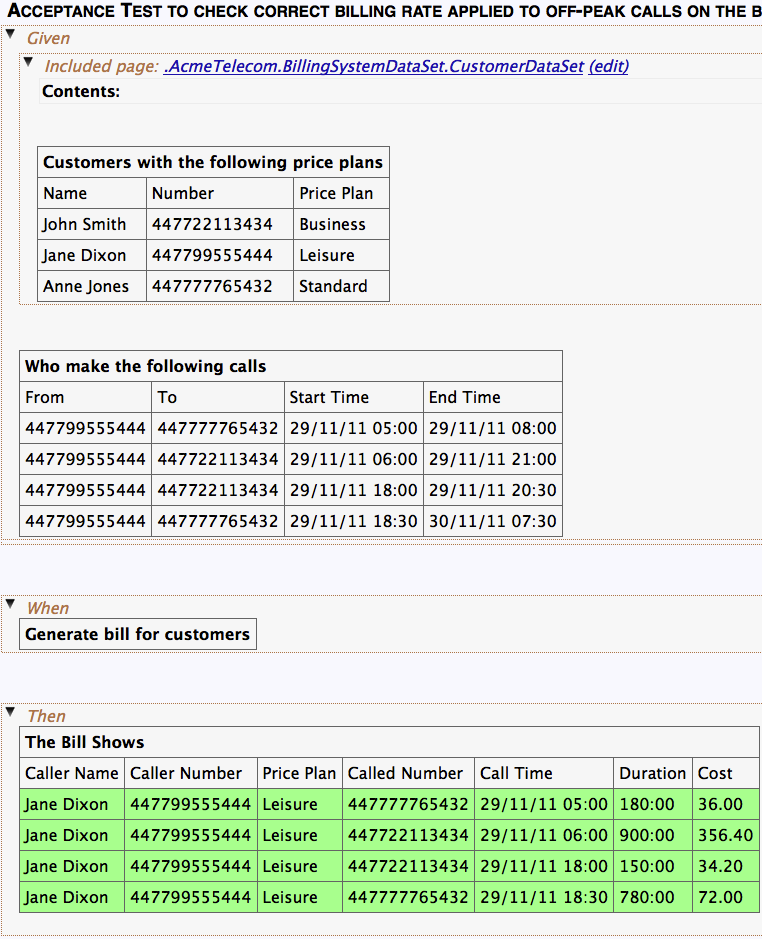
\includegraphics[scale=0.5]{images/fitnesse_test.png}
\end{center}

We established the call charges empirically by running the tests:
\\\\
\begin{tabular}{ l c c }
&				off-peak charges (pence/minute) &  peak charges (pence/minute) \\
business &		0.18&								0.18 \\
leisure & 			0.06& 								0.48 \\
standard & 		0.12&								0.30 \\
\end{tabular}

\pagebreak

\section{Unit Testing}

We started by implementing an Integration Test that provided a 'safety net' which prevented us from breaking existing functionality as we refactored the codebase. The Integration Test would set up a number of calls before requesting the bill for the customers. The existing system had not been written with testing in mind so it was very tricky for us to even introduce the Integration Test, let alone write unit tests or wire up FitNesse fixtures. 

The Integration Test initially had to depend on the external customer and tariff databases making it very brittle. Furthermore, calling createCustomerBills method of BillingSystem output to stdout and provided no way of sending values or verifying object interactions. In order to check the output bill we had to redirect System.out to a PrintStream, collecting the generated bill into a string on which assertions could be made. Another problem we encountered was that calls logged with the system would use the current time, making testing virtually impossible. In order to make the Integration Test pass we were forced to isolate this part of the code by introducing a seam. The seam was necessary to break dependencies and allow injection of test values. We we were confident that introducing this change to allow arbitrary times to be injected into CallStart and CallEnd would not change any behaviour of the system because we used IntelliJ IDEA's refactoring tools to do this. The following are code snippets resulting from making this initial change:

\begin{lstlisting}
billingSystem.callInitiated(caller, callee, startTime.getTime());

public CallStart(String caller, String callee, long timestamp) {
    super(caller, callee, timestamp);
}
\end{lstlisting}

Once we had the Integration Test passing, we started implementing new functionality using Test-Driven Development (TDD).  This allowed us to be confident in our changes, helped us build a suite of regression tests to be run on the CI server and made our code self documenting. The first few unit tests required us to refactor a fair amount of code to get them going green but, now that we had the integration test in place, we were able to verify that no behaviour had changed. We broke up large, complicated methods into smaller ones allowing for values to be sensed. We introduced seams by breaking dependencies and creating interfaces which could be mocked allowing for verification of object interactions. We expand on these points in the Refactoring section.

It's important to have good code coverage in the test suite as it ensures edge cases are covered and provides a regression test suite reducing the chance of future commits accidentally breaking behaviour . On completion of the task, we had 92\% line coverage across the whole project. The lines that were not covered were due to uncovered accessor or mutator methods and little coverage of HtmlPrinter for which we felt unit tests would be very brittle and pointless.

We used JUnit4 as our unit testing framework, Mockito for mocking objects and EMMA for gathering code coverage statistics. We used the Hamcrest library to create more readable assertions in our tests. We decided to use Mockito in place of JMock as we had more experience with it and it still provided a very cons ice and readable DSL.

\section{Refactoring}

We made heavy use of Dependency Injection (DI) when refactoring the system as it helped us decouple as many classes as possible, making the system more flexible to change. We provided interfaces for classes wherever there could be a sensible need to use alternative functionality. We could have gone one step further and used a DI framework such as Google Guice but decided against this because the object graph was very simple to set up and we felt such a framework would add some complexity with little benefit in this case. Instead, we tried to stick to the SOLID (Single responsibility, Open closed, Liskob substitution, Interface segregation and Dependency Inversion) principles wherever possible as they helped guide us in easy to read, extensible and maintainable code. Please see \url{http://www.natpryce.com/articles/000783.html} for a further discussion of why DI frameworks are not always a 'good thing'. Listed below is some of the refactoring we did:

\begin{itemize}
\item We introduced an interface for BillGenerator and and injected it into BillingSystem. It's role is to allow for different ways of formatting the bill and making this configurable is beneficial. For example, an DaytimePeriodGroupedBillGenerator may group calls into peak/off-peak or a CalleeOrderedBillGenerator may change the ordering of the calls to be by who the callee is.
\item Created a new BillingSystem test which would pass in a mock BillGenerator and verify that its send method is called with the correct arguments. In order to do the verify, equals and hashCode had to be implemented for LineItem, Call and CallEvent along with their respective tests.
\item We also decided to inject CustomerDatabase and TariffLibrary into the BillingSystem and again used mocking to create reliable tests as shown in the following snippet: 

\begin{lstlisting}[caption=Set up method in BillingSystemTest showing use of mock CustomerDatabase and TariffLibrary]
@Before
public void setUpCustomers() {
    MockitoAnnotations.initMocks(this);
    john = new Customer("John Smith", "447722113434", "Business");

    when(customerDatabase.getCustomers()).thenReturn(Arrays.asList(john));
    when(tariffDatabase.tarriffFor(john)).thenReturn(Tariff.Business);

    billingSystem = new BillingSystem(customerDatabase, 
    	tariffDatabase, billGenerator);
}
\end{lstlisting}

The Ports and Adapters design architecture could have been used to add a layer of abstraction between the system and the CustomerDatabase/TariffLibrary interfaces in case the library changes. We decided against it as the library is maintained internally at AcmeTelecom and not by a third party so we would be needlessly complicating the billing system.
\item Broke up the long createBillFor(customer) method into smaller methods such as calculateCostOf(calls) and calculateTotalBill(lineItems).
\item We noticed that BillGenerator's send method doesn't actually require totalBill as the LineItems already have the call cost from which the total can calculated. Therefore, we removed the argument and moved the totalBill calculation logic from the BillingSystem into the BillGenerator. We felt this is a reasonable assignment of roles as the BillingSystem is there to just calculate the cost for each call whereas what is shown on the bill is for BillGenerator to sort out.
\item Separated out the logic for calculating call costs into classes which implement a BillCalculator interface that provides a getCallCost(call, tariff). The FixedRateBillCalculator corresponded to the old billing requirement and we simply reused the existing logic to implement it. We added unit tests for this calculator but the acceptance tests only covered the new, variable rate calculation. If legislation ever changes such that customers need to be billed differently, all that would be required is a new implementation of BillCalculator that is injected into the BillingSystem. Here, we decided to use Setter Injection and provide a default VariableRateBillCalculator (explained in 'Implementing new requirements' section) in the constructor.
\item Reused the off-peak period logic and this remained in the DaytimePeakPeriod. The peak and off-peak start times can now be injected in the constructor. We also decided it was beneficial to have the DaytimePeakPeriod injected into the BillCalculators in case different logic was required for determining the peak period. We found that refactoring to use the JodaTime library came in handy here as it provides a very nice DSL for dealing with DateTime:
\\\\

\begin{lstlisting}[caption=The new offPeak(DateTime time) method showing the usage of the DSL provided by JodaTime]
final DateTime peakStart = new DateTime().withTime(7, 0, 0, 0);
final DateTime offPeakStart = new DateTime().withTime(19, 0, 0, 0);

public boolean offPeak(DateTime time) {
    boolean timeAfterOffPeakStart 
        = time.isEqual(offPeakStart) || time.isAfter(offPeakStart);
        
    return time.isBefore(peakStart) || timeAfterOffPeakStart; 
}
\end{lstlisting}

JodaTime also provides a simple way of both parsing and stringify-ing a DateTime according to some DateTimeFormat, meaning that it could be used to generate bills with the same date and time format as the existing system. Therefore, we decided to remove all uses of Timestamp and long and replaced them with JodaTime's DateTime which are easier to work with and have this nice descriptive DSL.
\item BillingSystem was split into CallLogger and BillingSystem as billing system originally had both of these roles breaking 'Single responsibility' principle in SOLID. The CallLogger is injected into the BillingSystem and is only used by it to getCallsFor(customer). This also introduces the possibility of extending the system with other types of CallLoggers such as one that can track a customer calling multiple people at the same time.
\item Restructured the system into three packages and removed the cyclic dependency between BillingSystem and BillGenerator (see below for before and after diagrams that were generated using Structure101).
\item Following these changes, the code for calculating a bill is greatly simplified and has been made a lot more readable:
\begin{lstlisting}
    private CallLogger callLogger;
    private CustomerDatabase customerDatabase;
    private TariffLibrary tariffDatabase;
    private BillCalculator billCalculator;
    private BillGenerator billGenerator;

    private void createBillFor(Customer customer) {
        List<Call> calls = callLogger.getCallsFor(customer);

        Tariff tariff = tariffDatabase.tarriffFor(customer);

        List<LineItem> items = calculateCostOf(calls, tariff);

        billGenerator.send(customer, items);
    }

    private List<LineItem> calculateCostOf(List<Call> calls, Tariff tariff) {
        List<LineItem> items = new ArrayList<LineItem>();

        for (Call call : calls) {
            BigDecimal callCost = billCalculator.getCallCost(call, tariff);
            items.add(new BillItem(call, callCost));
        }
        return items;
}
\end{lstlisting}
\pagebreak

\end{itemize}

Structure before refactoring:
%Diagram before
\begin{center}
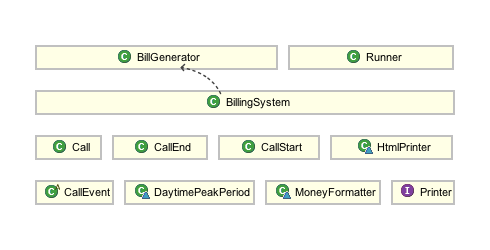
\includegraphics[scale=0.75]{images/original_structure.png}
\end{center}

Structure after refactoring demonstrating the layering in the new system:
%Diagram after
\begin{center}
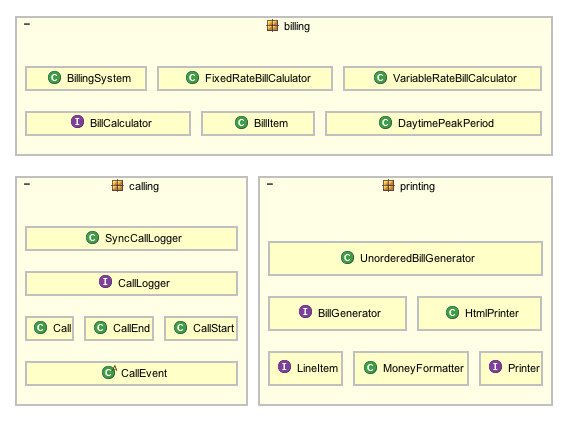
\includegraphics[scale=0.75]{images/new_structure.png}
\end{center}

\section{Implementing new requirements}
This boiled down to just providing a new implementation for BillCalcuator that to the new, variable billing requirement as laid out in the specification. We did this by creating a VariableRateBillCalcuator that provides a getCallCost(call, tariff) and internally uses a nextPeakChange(currentTime) to calculate what portion of a call is during peak or off-peak times.

Unit tests helped guide the development of this class and without them we could have easily missed corner cases such as a call that starts at 07:00/19:00 or a call that starts during one day but ends on the next. The acceptance tests all passed following the implementation of this class and configuration of BillingSystem to use it over the old calculator.

%Anything else you did
\section{Development Process}
We used the Git distributed version control system to allow our team to effectively collaborate on the same code, hosting our repository on Github as they offer a reliable service and free accounts for students. 

We used a free micro instance on Amazons Elastic Compute Cloud (EC2) to set up the free Jenkins Continuous Integration (CI) system. Every commit to git would trigger Github's post web hooks, alerting Jenkins that there had been a commit. Jenkins would then checkout the code, build it, run the acceptance tests using FitNesse, Integration and Unit tests using JUnit and finally generate code coverage with EMMA. We could also see the status of the builds of all commits along with their code coverage and test status using the Jenkins web interface. Every time the build status changed, e.g. a failed build after a successful build, an email would be sent to the group as a warning. Using continuous integration enabled the group to track our progress towards a system with full code coverage and then ensure that we maintained the coverage as we made changes. It helped to add momentum to the development process as we all aimed for high code coverage and to keep the build green. Below is a screenshot of the project page on Jenkins web interface with testing and code coverage graphs:
\\

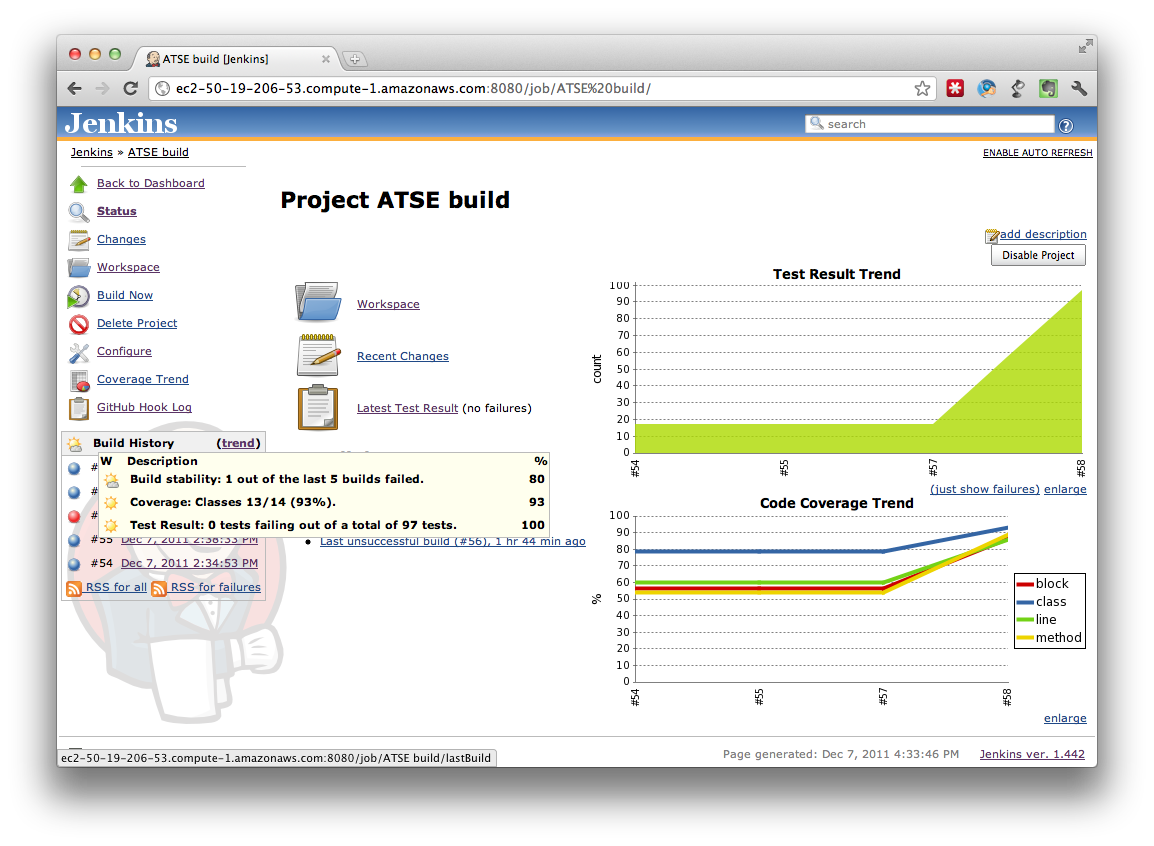
\includegraphics[scale=0.4]{images/jenkins_project.png}
\\

To manage building and other tasks associated with the project we used Gradle. It has a nice DSL for build tasks and is very flexible as it allows the use of Ant build tasks and Maven repositories if required. Java build targets were set up by simply including the java plugin although we had to add a main class attribute to the jar manifest file. We also used the emma plugin so that every time we built and ran the tests, EMMA code coverage statistics were generated for Jenkins to use. Lastly we used the idea plugin which allowed us to generate Intellij IDEA project files which had the libraries and build targets predefined and in sync with Gradle.

When FitNesse tests failed we had to use Java's remote debugging from within IntelliJ to attach to its process. This allowed is to use all the standard IntelliJ debug tools (breakpoints, stepping through code, variable inspection) to resolve the issue causing the bug.

\pagebreak

\section{Future Improvements}

\begin{itemize}
\item Define default charging behaviour for calls that last less than e.g. a second. Perhaps there should be a minimum charge?
\item Extend CallEvent to allow for more description of the calls, e.g hangup events and hold events.
\item Implement a new CallLogger that can track a user making multiple calls at the same time
\item Provide a new BillGenerator that produces PDF bills using a PdfPrinter and then emails them to the customer.
\item Possibly implementing a DSL to be used in tests for creating customers or calls. The group decided against this seeing as the problem domain is relatively simple to understand.
\end{itemize}

If these future improvements were to be added the same development methodology could be used as it will scale with increasing numbers of developers and commits. That said, there are a number of improvements we would make:
\\

\textbf{Infrastructure hosting}: The git repository and Jenkins deployment would have to be hosted on AcmeTelecom's own servers for greater security and so that builds would run much faster.

\textbf{Continuous Deployment}: To deploy the system we would extend the current CI system to automatically promote the new builds to production. Deployments could simply correspond to folders with a symlink to the latest version allowing for blue/green releasing or an update system to push the software to the users.

\textbf{Code Quality:} Jenkins picks up all the functional shortcomings of commits when it runs the various testing frameworks. Subjective matters, such as code style and implementation details, typically can't be vetted easily and having formal code review upon commit using a Jenkins plugin such as gerrit would be beneficial. This wasn't a problem as we were a small group and any bad code was noticed quickly. To ensure bad commits don't make it into the repository it would also be a good idea to use 'remote-runs' where change lists are only committed if they build successfully.

\textbf{Registering issues:} If the system is under continued development it would make sense to record bugs and features to implement in an issue tracking and review system such as JIRA. This software manages the flow of issues as they get listed, picked up by a developer, implemented or fixed and then finally closed. 

Making these changes would ensure that the development of the system scales and the quality of the changes are high.

\end{document}